%----------------------------------------------------------------------------
% Start
%----------------------------------------------------------------------------

\documentclass{article}

\usepackage{graphicx} % Required for the inclusion of images
\usepackage{tocloft}
\usepackage[nottoc,numbib]{tocbibind} % Reference in TOC and numbered
\usepackage{url} % Reference include URL

\renewcommand{\cftsecleader}{\cftdotfill{\cftdotsep}}
\renewcommand{\labelenumi}{\alph{enumi}.}

\setlength\parindent{0pt} % Removes all indentation from paragraphs


%----------------------------------------------------------------------------
% Document Information
%----------------------------------------------------------------------------

\begin{titlepage}

\title{Giguesaur: Game Logic}
\author{Ashley Manson}
\date{\today}

\begin{document}
\maketitle

\begin{center}
\large
Co-Workers: Joshua La Pine \& Shahne Rodgers\\
Supervisors: Geoff Wyvill \& David Eyers\\

\vspace*{1\baselineskip} % Skip a line

Dept. of Computer Science\\
University of Otago
\end{center}

\end{titlepage}

%----------------------------------------------------------------------------
% Table of Contents
%----------------------------------------------------------------------------

\tableofcontents
\newpage

%----------------------------------------------------------------------------
% Introduction
%----------------------------------------------------------------------------

\section{Introduction}

Our vision for our completed Giguesaur application was allowing a classroom of children, each with their their own iPad, to run around and solve a jigsaw puzzle together. Imagine a classroom full of kids where they are all trying to work on a single conventional jigsaw puzzle; such a scheme is in no way pratical. The main goal of our project, besides all the design and technical subgoals, is simply to make a that is fun for children to play and work together.

% Overview of the project
\subsection{Overview}
The Giguesaur application development was divided into three different components. Joshua La Pine was in charge of developing the computer vsion part of the project, which allows for the puzzle pieces to be rendered over top the 'game board' in the real world. Shahne Rodgers took charge of the networking component of the project, which was crucial in allowing more than one player to interact with the jigsaw puzzle. Finally my part of the project was to develop the game logic and render the game to the iPad's screen.

% Background including what a puzzle is and other games
\subsection{Background}
There are many jigsaw puzzle games that are available for iOS and other hand-held devices, such as Magic Jigsaw Puzzles \cite{ref:MagicJigsaw} and Jigsaw Puzzle \cite{ref:JigsawPuzzle}, but the majority of them are limited in the way they look due to them using an orthographic projection to render the jigsaw puzzles. What this projection means is that the puzzle pieces of the jigsaw puzzle are flat on the screen, the player can only look at the jigsaw puzzle from top down, there is no depth and all the puzzle pieces are displayed as the same size. This is something that does not work for the Giguesaur project as the puzzle pieces are rendered in a perspective projection, so when the jigsaw puzzle is rendered onto the game board it looks more realistic, as puzzle pieces that are further away from the camera are shown to be smaller than pieces that are closer to the camera. Another limitation of jigsaw puzzle games is the way they can be interacted with, by which I mean the way they can be solved. The puzzle pieces have to be placed into a predefined grid. Farms And Animals Puzzles \cite{ref:FarmPuzzle} is an example of a game that has this grid layout for the puzzle pieces to be placed in, which is shown in figure \ref{fig:FarmsAnimals}, it also shows the limited orthographic perspective of the game. This means that all the puzzle pieces will be placed in the centre of the screen. This is something that was illogical for the project and I did not want to limit the scope of the game. I have made it possible for the jigsaw puzzle to be solved anywhere on the board, be it in the centre of the game board or off in a corner of the game board. I also believe that it makes for a more interesting game.

\begin{figure}[ht]
\begin{center}
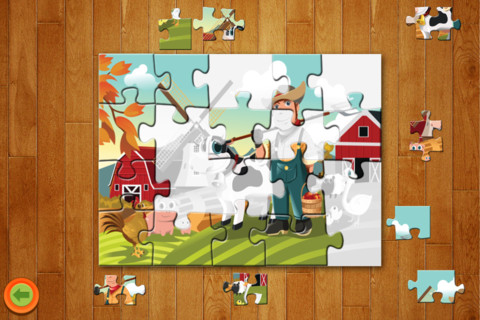
\includegraphics[width=0.85\textwidth]{images/FarmAnimalsJigsawImage}
\caption{Screenshot of Farms And Animals Puzzles \cite{img:FarmPuzzle}.}
\label{fig:FarmsAnimals}
\end{center}
\end{figure}

% iOS compared to Android
\subsection{iOS} % Needs rewritten <<<<<<<<<<<<<<<<<<<<<<<<<
iOS is operating system paradim ran on Apples small number of hand held devices, which are similar in many ways such as hardware and software implementaions.. It is considered to be held to a higher standard compared to Android, of which is ran on large number of devices crossing multiple different versions of the operating system, with a wide range of screen resoultions and processing power, which is due to the open source nature of the operating system. We had decided that the Gigusaur game would be developed on the iOS platform for a couple of reasons. iOS hardware was more standardized than Android, as Apple are the only developers of iPhones and iPads it made it easy for us to write the code, knowing that we would be relativly safe that what we developed would work on the majority of iOS devices, at least the ones with cameras. We couldn't be certain that any Android development of an application would work, nor would it have been possible for a forth year project to ensure that the application would have worked on kinds of Android devices. iOS itself is also less fragmented piece of software compared to Android, as Android is run a multiple of different devices, we would of had to accomadate for a lot more unknown variables that we neccessarily did not have the time for. Apple also has a sophisticated tool that helped us tremendously with the developing of the app, which was the integrated development enviornment XCode. XCode allowed us to rapidly develop the Giguesaur application with ease, and had a lot of helpful software to help with the development such as profiling of the running application.

% Brief explaination of AR and examples
\subsection{Augmented Reality}
Augmented reality is the idea of superimposing virtural objects on top of the real world in a realistic way the looks convincing enough for someone to believe what they are seeing is actually real. In figure \ref{fig:ARDefender} is shows a game world being played on a simple coffee table. The game is a simple tower defence where the user aims where the tower shoots by moving the iPhone around the table while the camera has the marker on the table in view. The marker on the table, of which is hidden under the projection of the defence tower, is what allows the game to get the required information to correctly pose the game objects onto the table.

\begin{figure}[ht]
\begin{center}
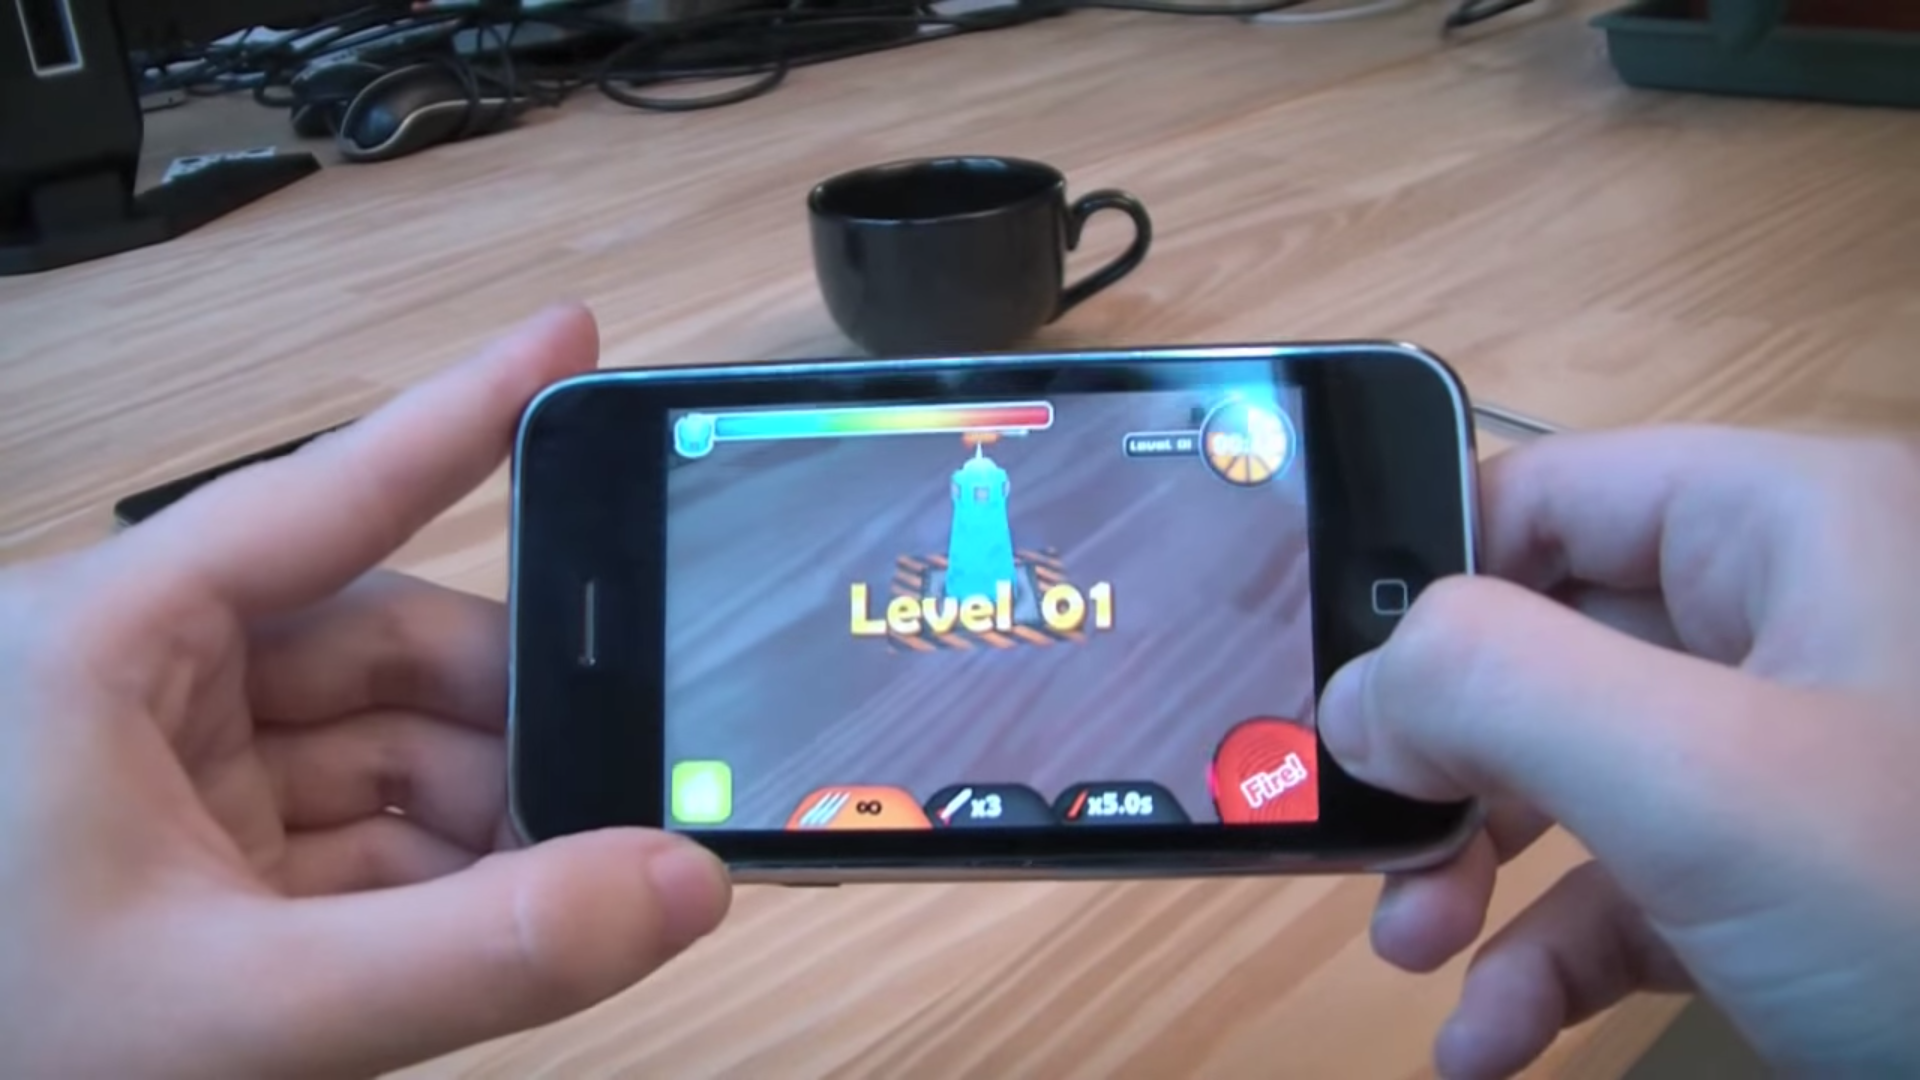
\includegraphics[width=0.85\textwidth]{images/ARDefenderImage}
\caption{Screenshot of ARDefender \cite{img:ARDefender}.}
\label{fig:ARDefender}
\end{center}
\end{figure}

% Brief introduction on my work
\subsection{Game Logic}
As I stated previously, I was in charge of developing the game logic for the Giguesaur game. This meant I had to create the logic for how jigsaw puzzle pieces interacted with each other and how the user interacted with the game. The jigsaw puzzle is made up of a grid with a specific number of rows and columsn. Each piece has four edges, and an edge either has a neighbouring piece or not. An edge of a piece can be open, meaning it has not joined to its neighbour currently or closed meaning it has joined to its neighbour currently, or if the edge has no neighbour it is invalid, meaning it can't join or be joined to another piece for that edge. An invalid edge would be the outside edge of the puzzle. Each piece of the puzzle has a unique ID, a position in space, or an x, y coordinate on the board, and a rotation with a value between 0 and 360 degrees. This is how I developed the game logic. I made up my own data structure to store these details, the ID determines the index of the array of pieces where the piece is held, the x, y coordinate determines where on the board the piece is displayed and the rotation affects the orientation of the piece. The board that the pieces are placed on has a width and length, which are along the x, y axis, which confines where the puzzle pieces can be placed, as all the pieces have an x, y coordinate. 

%---------------------------------------------------------------------------
% Work Done
%---------------------------------------------------------------------------

\section{Work Done}

% Work done on Mac
\subsection{Prototype}
In the beginning of the project I proceded to develop a prototype of the Giguesaur game on the Mac, using some simple OpenGL to render the game. Working on the Mac helped when I was creating the game logic for the application.

\begin{figure}[ht]
\begin{center}
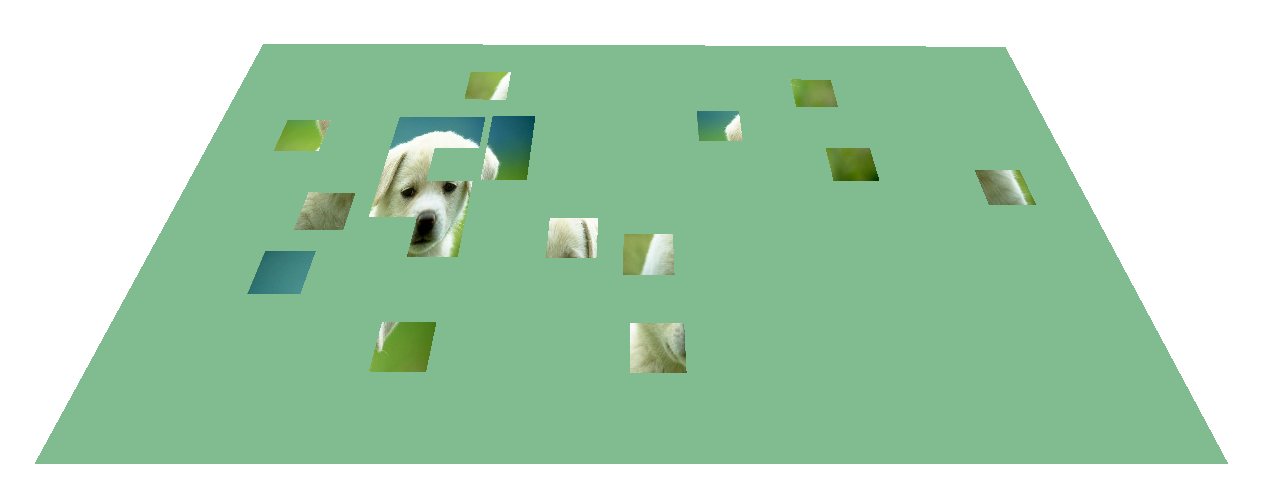
\includegraphics[width=1\textwidth]{images/MacBuildImage}
\caption{Screenshot of Prototype Build on the Mac.}
\label{fig:MacBuild}
\end{center}
\end{figure}

% What the game can do
\subsection{Game Mechanics}
I wanted to enable a feature that allowed pieces to snap together, meaning if a piece was in a specified range to its neighbour, the piece being placed back on the board would move so that the two piece were right next to each other, or they snapped together, which is shown in the Java Jigsaw Puzzle game made by Centurio \cite{ref:SourceJigsaw}. This also has the added bonus of making it easier to check if pieces are right next to each other, rather than relying on the user to carefully place pieces together. How the check is made to see if two pieces should snap together is by comparing the distances between the corresponding corner points, and if the distances are less than the snap variable, the pieces snap together. So if the piece being put back on the board is being snapped to its left neighbour piece, the original piece top left point and the neighbours top right point would be checked, as well as the original piece bottom left point and the neighbour's bottom right point would be checked. The reason two distances are checked is to make sure that piece rotations are taken into consideration when snapping pieces together, so as avoid an unusual snap where a piece rotated 90 degrees snaps to its neighbour not rotated. When a piece is snapped to another piece, the piece saves the rotation of its neighbour as its own, so that when the change is rendered, they both have the same rotation when beside each other. For a puzzle to be considered solved, all the pieces should be snapped to their corresponding neighbours. Once a piece has snapped to its neighbour, a variable for that edge is set as closed, as well as the neighbour's edge. So if a piece has snapped to its right neighbour, its right edge is set as closed and the neighbour's left edge is set as closed. The check to see if the puzzle has been solved goes through all the pieces' edges to see if they are all closed.

% Porting to iPad including changes and problems incountered
\subsection{Port to iPad}
Once I had established a working prototype for the Mac, the next step was to port the code to an iPad.

\begin{figure}[ht]
\begin{center}
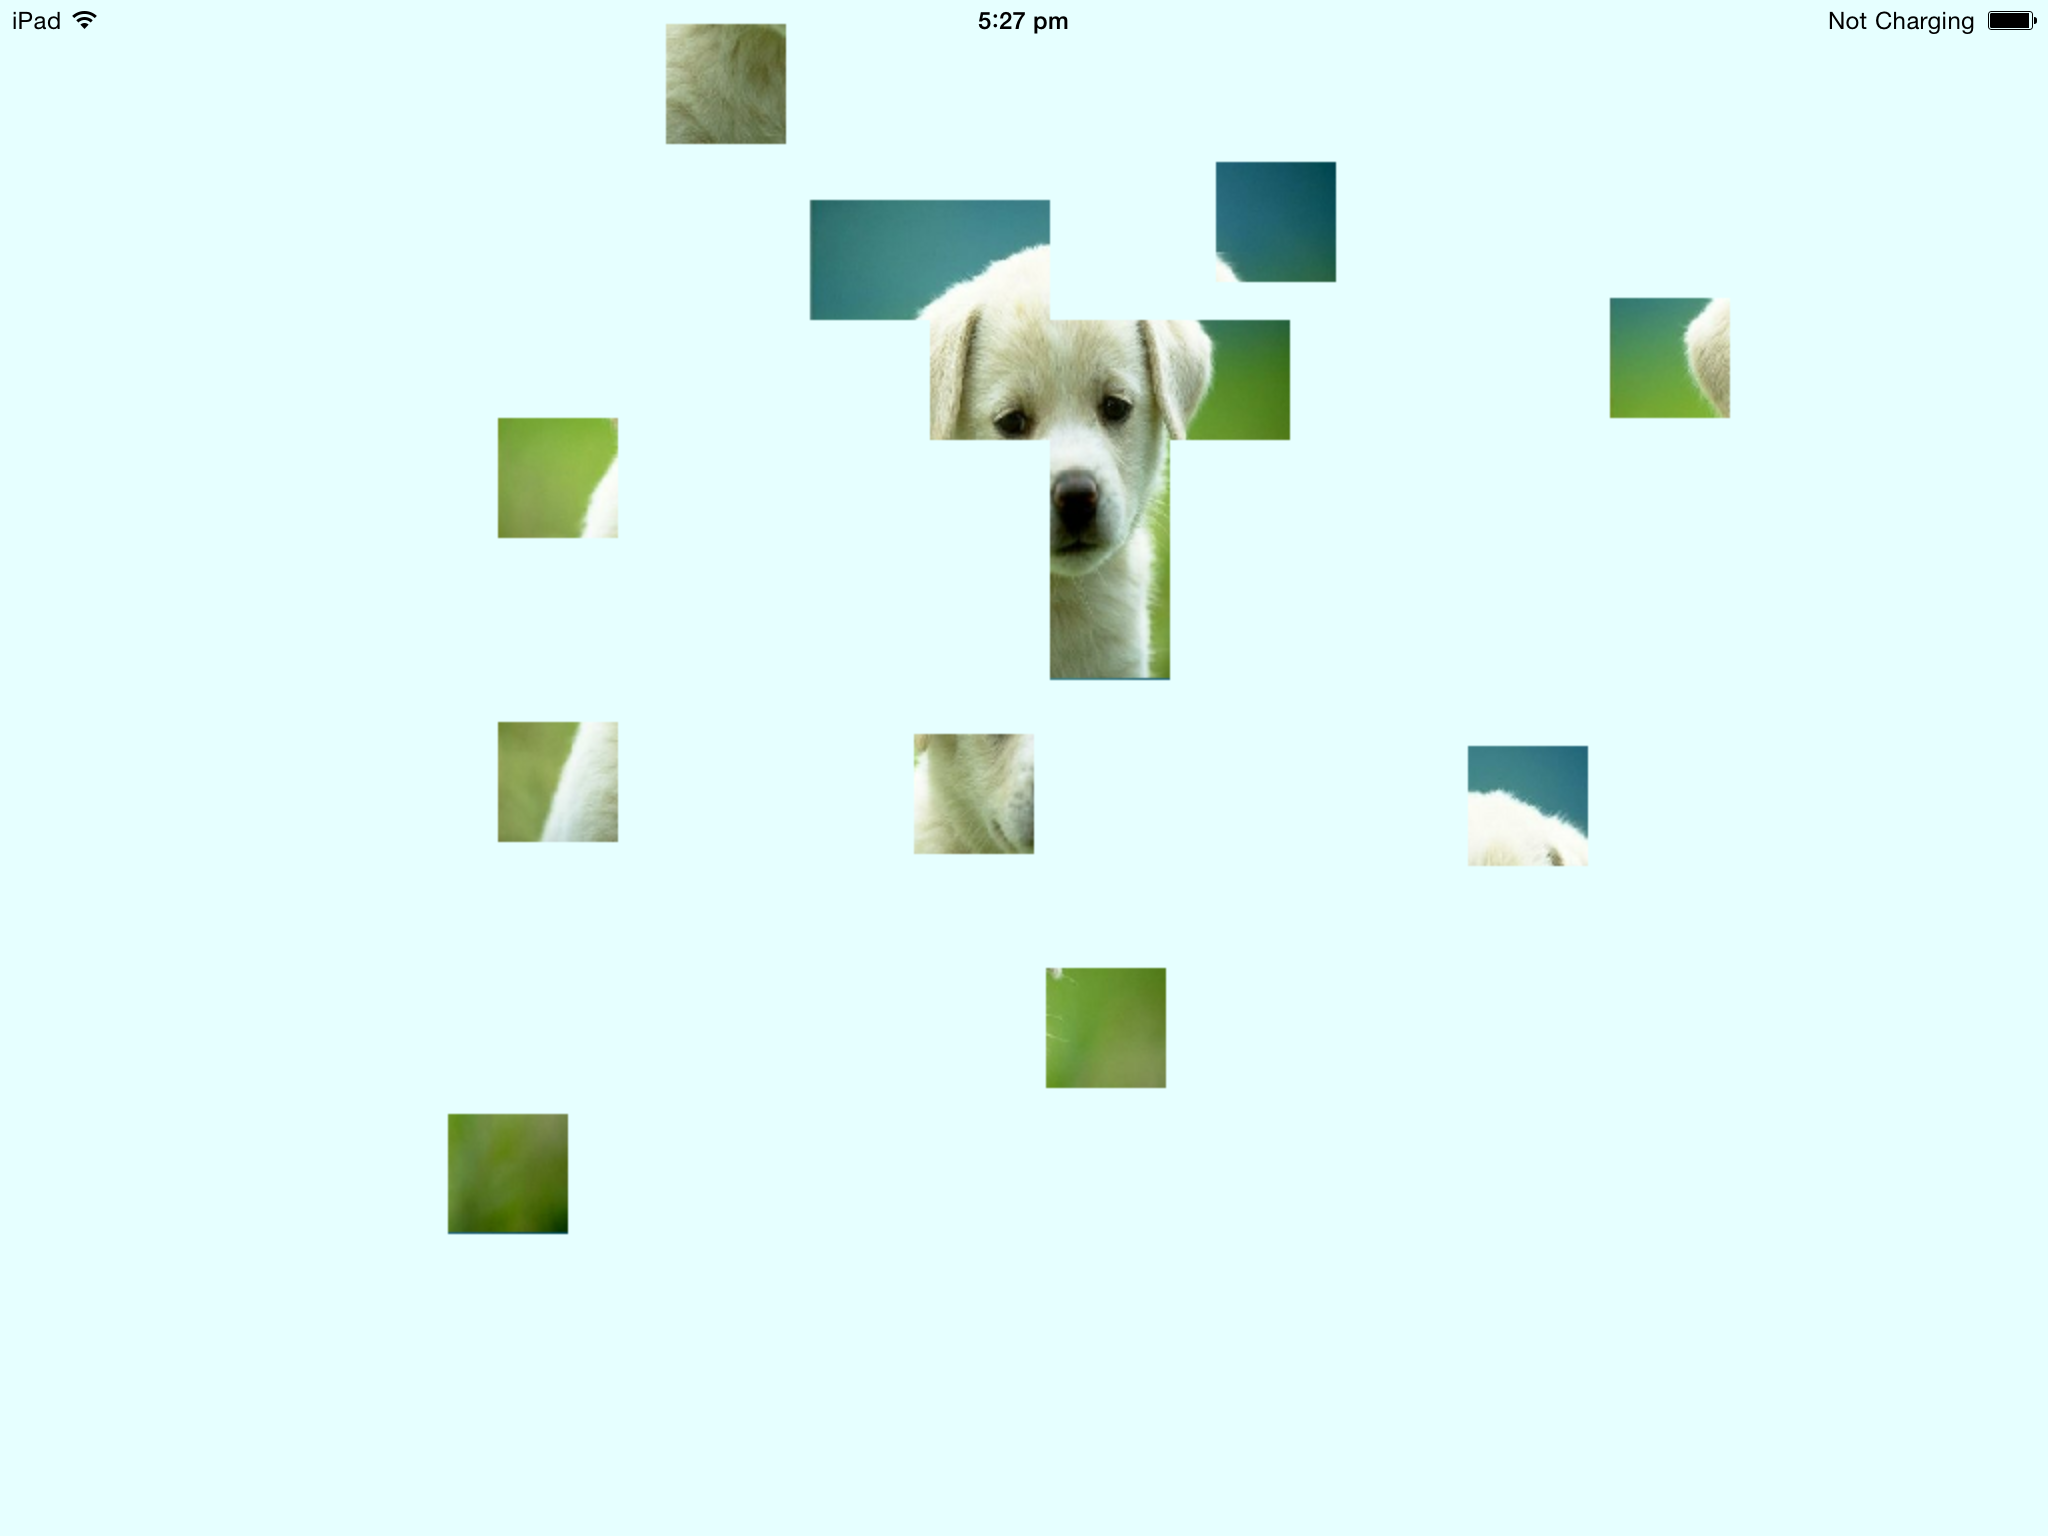
\includegraphics[width=0.85\textwidth]{images/iPadPortImage}
\caption{Screenshot of the first port to iPad.}
\label{fig:iPadPort}
\end{center}
\end{figure}

% Renderind and moving pieces
\subsection{Rendering}
The first major goal was to have a jigsaw puzzle rendered to the screen and the ability to move the jigsaw puzzle pieces around. I used OpenGL to do all the rendering of the jigsaw puzzle, using the coordinates of the jigsaw puzzle pieces, their current rotation and side length of the puzzle pieces as parameters to get them displayed correctly. With the parameters of each of the puzzle pieces, I get the four coordinates of their corners, with these I pass them to OpenGL and the puzzle pieces are rendered to the screen.\\
To pick up a piece the user taps the image of the piece on the screen. That piece that the user has tapped is then stored in the users “inventory” and they are no longer able to pick up another piece, until they have placed the piece that they are holding back onto the board. The inventory is just a term I am using to state if the user is holding or not holding a piece, meaning it can be easily checked to see if it is empty or not. This is also allows me to increase the storage space of the inventory later on in the project if I wish to allow the user to hold more than one piece. Currently the inventory is displayed in the lower left corner of the screen, meaning the user can see if they are holding a piece or not. The screen x, y coordinate from a finger tap are converted to a board x, y coordinate. If this is close enough to a piece then that piece is added to the user's inventory. This allows for the board to be rendered with a perspective projection, making the scene more realistic and achieving the augmented reality feel.

% Integrating with others including problems incountered
\subsection{Integration}
After I had succesfully ported the application to the iPad and had eveything from the prototype working correctly, we as a team had to work together on integrating all three parts of the project into a single coherent piece of software. The main issue we all quickly found out was that this task proved to be more difficult than previously thought. 

%---------------------------------------------------------------------------
% Results
%---------------------------------------------------------------------------

\section{Results}
The finished product is a fully functional, interconected, jigsaw puzzle solving game.

\begin{figure}[ht]
\begin{center}
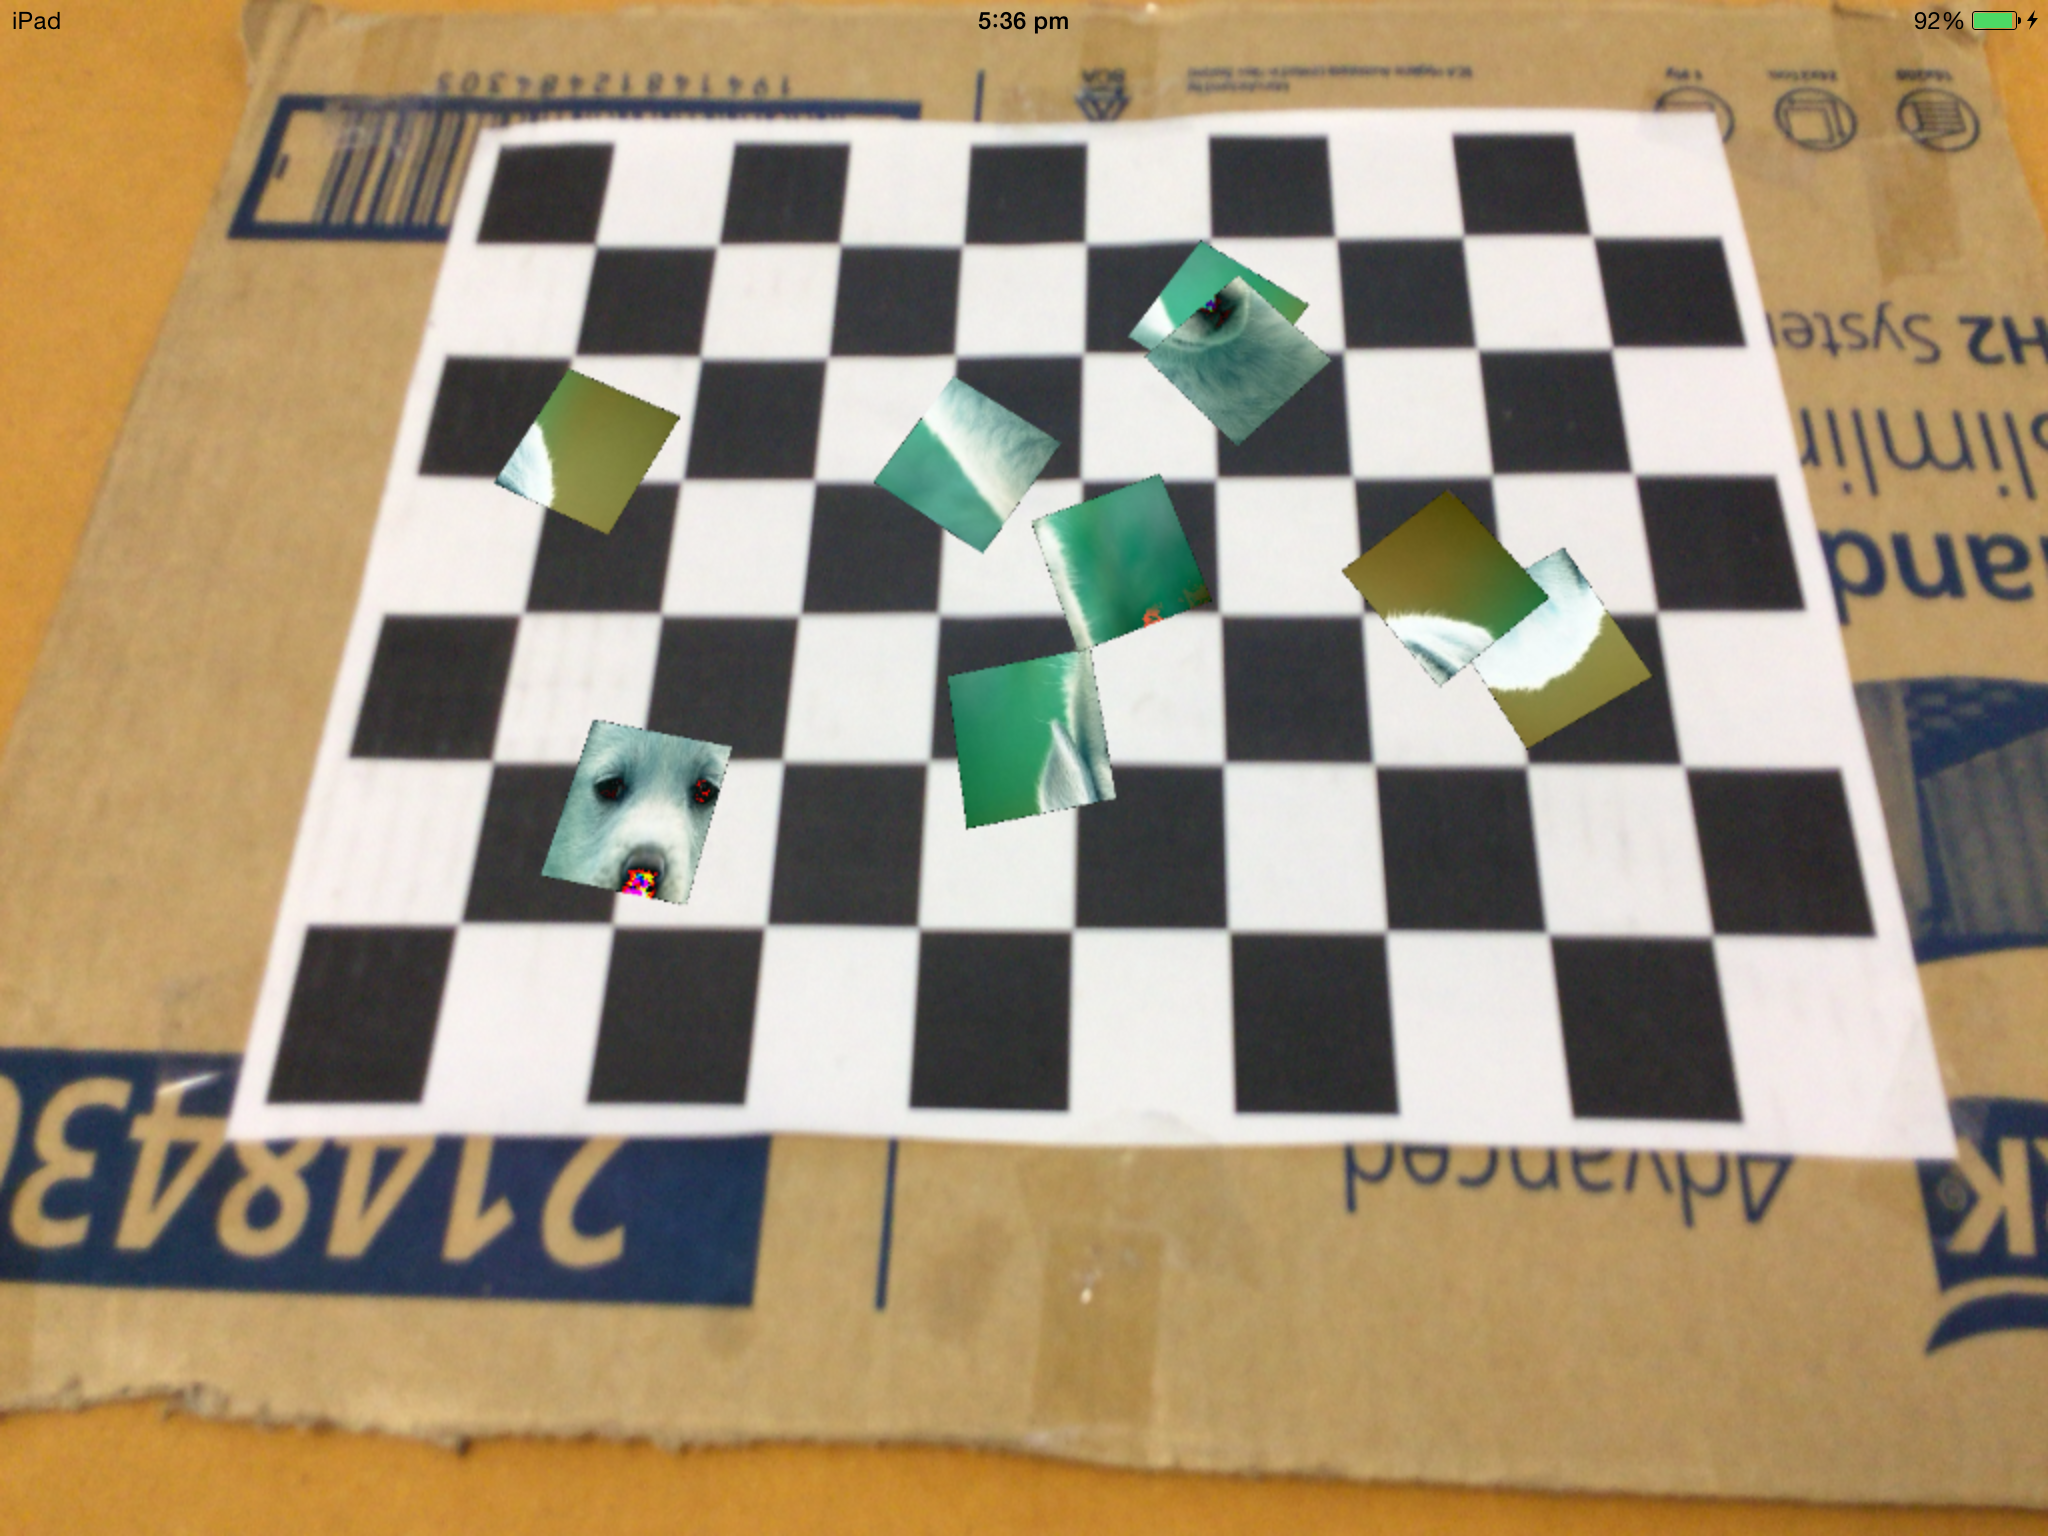
\includegraphics[width=0.85\textwidth]{images/iPadFinalImage}
\caption{Screenshot of the final build running on a iPad.}
\label{fig:iPadFinal}
\end{center}
\end{figure}

%---------------------------------------------------------------------------
% Conclusion
%---------------------------------------------------------------------------

\section{Conclusion}

% What the thing looks like
\subsection{Final Build}

% What hasn't been done
\subsection{Future Work}

\subsection{Final Words}

%---------------------------------------------------------------------------
% References
%---------------------------------------------------------------------------

\clearpage
\bibliographystyle{ieeetr}
\bibliography{references}

%---------------------------------------------------------------------------
% End
%---------------------------------------------------------------------------

\end{document}
